\documentclass[11pt, a4paper]{article}

\usepackage[english]{babel}
\usepackage{sleek}
\usepackage{common}

\title{Introduction to Artificial Intelligence (INFO8006)}
\subtitle{Exercise session 7}

\begin{document}

\maketitle

\begin{thbox}{Markov decision processes}
    A \thighlight{Markov decision process} is a tuple ($\mathcal{S}, \mathcal{A}, P, R$) such that:
    \begin{itemize}
        \item $\mathcal{S}$ is a set of \thighlight{states} $s$;
        \item $\mathcal{S}$ is a set of \thighlight{actions} $a$;
        \item $P$ is a (stationary) \thighlight{transition model} such that $P(s'\mid s,a)$ denotes the probability of reaching state $s'$ if action $a$ is done in state $s$;
        \item $R$ is \thighlight{reward function} that maps immediate (finite) reward values $R(s)$ obtained in states $s$.
    \end{itemize}
\end{thbox}

\begin{thbox}{Bellman equation}
    The \thighlight{utility} of a state is the immediate reward for that state, plus the expected discounted utility of the next state, assuming that the agent chooses the optimal action:
    $$
    V(s) = R(s) + \gamma \max_a\sum_{s'}P(s'\mid s,a)V(s').
    $$
\end{thbox}

\begin{thbox}{Value/policy iteration}
    The \thighlight{value iteration} algorithm provides a fixed-point iteration procedure for computing the state utilities $V(s)$. By denoting $V_i(s)$ the estimated utility at iteration $i$ and starting from an initial guess $V_0(s)$, we update the estimates to be consistent with \thighlight{Bellman equation}:
    $$
    V_{i+1}(s) = R(s) + \gamma \max_a\sum_{s'}P(s'\mid s,a)V_i(s')
    $$
    which always converges for $\gamma < 1$.\\

    The \thighlight{policy iteration} algorithm instead directly computes the \thighlight{policy} $\pi$ by alternating between \thighlight{value evaluation} under the current \thighlight{policy} estimate
    $$
    V_i = V^{\pi_i}
    $$
    and \thighlight{policy} improvement
    $$
    \pi_{i+1}(s) = \arg \max_a \sum_{s'}P(s' \mid s,a) V_i(s').
    $$
\end{thbox}

\begin{thbox}{Reinforcement learning}
    \thighlight{Reinforcement learning} is used in unknown MDP, i.e. MDP where the \thighlight{transition model} and the \thighlight{reward function} are unknown. The goal is still to extract the optimal \thighlight{policy} by observing or interacting with the environment in order to jointly learn these dynamics and act upon them.\\
    RL can be decomposed in \thighlight{model-based} and \thighlight{model-free} methods. The former estimates explicitly the environment and then use this estimation as the empirical MDP whereas the latter do not model the environment explicitly.
\end{thbox}

\begin{thbox}{Temporal-difference learning}
    \thighlight{Temporal-difference learning} consists in updating $V^\pi(s)$ each time the agent experiences a transition $(s,r,a,s')$ under a policy $\pi$.\\
    When a transition from $s$ to $s'$ occurs, the temporal-difference update steers $V^\pi(s)$ to better agree with the Bellman equations for a fixed policy, i.e.
    $$
    V^\pi(s) \leftarrow V^\pi(s) + \alpha(r + \gamma V^\pi(s') - V^\pi(s))
    $$
    where $\alpha$ is the \thighlight{learning rate}.
\end{thbox}

\begin{thbox}{Q-Learning}
    By defining \thighlight{Q-values} as $V(s) = \max_a Q(s,a)$, we have
    $$
    Q(s,a) = R(s) + \gamma \sum_{s'} P(s'\mid s,a) \max_{a'}Q(s',a').
    $$
    The state-action-values $Q(s,a)$ can be learned in a model-free fashion using a temporal-difference method known as \thighlight{Q-Learning}. Q-Learning consists in updating $Q(s,a)$ each time the agent experiences a transition. The update equation for TD Q-Learning is
    $$
    Q(s,a) \leftarrow Q(s,a) + \alpha(r + \gamma \max_{a'}Q(s',a') - Q(s,a)).
    $$   
\end{thbox}
\textbf{In session exercises}: Ex. 1, Ex. 4
\newpage

\part{Making decisions}

\section{Micro-Blackjack (UC Berkeley CS188, Spring 2014)}

In Micro-Blackjack, you repeatedly draw a card (with replacement) that is likely to be a 2, 3 or 4. At each step, if the total score of the cards is lower than 6, you can either \enquote{draw} ($d$) or \enquote{cash} ($c$). Otherwise, you can only cash. When you cash, the game stops and your utility is equal to your total score (up to 5) plus 1, or zero if you get a total of 6 or higher. Until you cash and after it, you receive no reward. There is no discount ($\gamma = 1$).

\begin{enumerate}
    \item Formalize Micro-Blackjack as an MDP.

    \begin{solution}
        A Markov decision process (MDP) is a tuple $(S, A, P, R)$, where $S$ is a set of reachable states, $A(s)$ is a set of available actions, $P(s' | s, a)$ is a (stationary) transition model and $R(s)$ is a reward function.

        In our case,
        \begin{align*}
            S & \subset \mathbb{N} \times \cbk{0, 1} \\
            A(s = (s_1, s_2)) & = \begin{cases}
                \cbk{d, c} & \text{if } s_1 < 6 \text{ and } s_2 = 0 \\
                \cbk{c} & \text{if } s_2 = 0 \\
                \cbk{} & \text{otherwise}
            \end{cases} \\
            P(s' = (s_1', s_2') | s = (s_1, 0), a) & = \begin{cases}
                1 & \text{if } s_1' = s_1 \text{ and } s_2' = 1 \text{ and } a = c \\
                \frac{1}{3} & \text{if } s_1' - s_1 \in \cbk{2, 3, 4} \text{ and } s_2' = 0 \text{ and } a = d \\
                0 & \text{otherwise}
            \end{cases} \\
            R(s = (s_1, s_2)) & = \begin{cases}
                s_1 + 1 & \text{if } s_1 < 6 \text{ and } s_2 = 1 \\
                0 & \text{otherwise}
            \end{cases}
        \end{align*}
    \end{solution}

    \item Derive the optimal policy for this MDP.

    \begin{solution}
        Let $(s_0, s_1, \dots, s_l)$ be a sequence of states, \ie{} a path. Its utility is
        \begin{equation*}
            \sum_{t = 0}^{l} \gamma^t R(s_t),
        \end{equation*}
        where $\gamma \in (0, 1]$ is the discount factor. For a policy $\pi : S \mapsto A$ to be optimal, it should maximize its \emph{expected} utility
        \begin{align*}
            V^\pi(s_0) & = \E \sbk*{\sum_{t = 0}^\infty \gamma^t R(s_t)} \\
            & = R(s_0) + \gamma \, \E \sbk*{V^\pi(s_1)} \\
            & = R(s_0) + \gamma \sum_{s_1} P(s_1 | s_0, \pi(s_0)) V^\pi(s_1),
        \end{align*}
        where the states $s_{t+1} \sim P(s | s_t, \pi(s_t))$. Therefore, we define the value $V(s)$ of a state $s$ is its maximum expected utility, \ie{}
        \begin{align*}
            V(s) & = V^{\pi^*}(s) \\
            & = \max_\pi V^\pi(s) \\
            & = \max_\pi R(s) + \gamma \sum_{s'} P(s' | s, \pi(s)) V^\pi(s') \\
            & = R(s) + \gamma \max_\pi \sum_{s'} P(s' | s, \pi(s)) V^\pi(s') \\
            & = R(s) + \gamma \max_{a \in A(s)} \sum_{s'} P(s' | s, a) \max_\pi V^\pi(s') \\
            & = R(s) + \gamma \max_{a \in A(s)} \sum_{s'} P(s' | s, a) V(s') ,
        \end{align*}
        where $\pi^*$ is the optimal policy
        \begin{align*}
            \pi^*(s) = \arg \max_{a \in A(s)} \sum_{s'} P(s' | s, a) V(s') .
        \end{align*}

        To find this optimal policy, we can apply either the \emph{value iteration} or \emph{policy iteration} algorithms.

        \begin{itemize}
            \item In value iteration, we estimate the value $V(s)$ by value estimates $V_i(s)$ and update them with the Bellman operator
            \begin{equation*}
                V_{i+1}(s) = (B V_i)(s) = R(s) + \gamma \max_{a \in A(s)} \sum_{s'} P(s' | s, a) V_{i}(s')
            \end{equation*}
            until convergence ($V_{i + 1} = V_i$). For our task, it should be noted that all states $s = (s_1, 1)$ are terminal, meaning that they don't allow to take any actions. Consequently, the value of these states is exactly their reward, \ie{}
            \begin{equation*}
                V(s = (s_1, 1)) = R(s) .
            \end{equation*}
            Let $V_0(s) = R(s)$ be our first value estimate.

            \begin{table}[h]
                \centering
                \begin{tabular}{c|cccccc|cccccc}
                    \toprule
                    $s_1$    & 0 & 2 & 3 & 4 & 5 & $6+$ & 0 & 2 & 3 & 4 & 5 & $6+$ \\
                    $s_2$    & \multicolumn{6}{c|}{0}   & \multicolumn{6}{c}{1}    \\
                    \midrule
                    $V_0(s)$ & 0 & 0 & 0 & 0 & 0 & 0    & 1 & 3 & 4 & 5 & 6 & 0    \\
                    $V_1(s)$ & 1 & 3 & 4 & 5 & 6 & 0    & 1 & 3 & 4 & 5 & 6 & 0    \\
                    $V_2(s)$ & $\frac{12}{3}$ & $\frac{11}{3}$ & 4 & 5 & 6 & 0 & 1 & 3 & 4 & 5 & 6 & 0 \\
                    $V_3(s)$ & $\frac{38}{9}$ & $\frac{11}{3}$ & 4 & 5 & 6 & 0 & 1 & 3 & 4 & 5 & 6 & 0 \\
                    $V_4(s)$ & $\frac{38}{9}$ & $\frac{11}{3}$ & 4 & 5 & 6 & 0 & 1 & 3 & 4 & 5 & 6 & 0 \\
                    \bottomrule
                \end{tabular}
            \end{table}

            Each iteration of this algorithm takes $\mathcal{O}(\abs{S}^2 \abs{A})$ operations.

            \item In policy iteration, we estimate the optimal policy $\pi^*$ by policy estimates $\pi_i$ and update them with
            \begin{equation*}
                \pi_{i+1}(s) = \arg \max_{a \in A(s)} \sum_{s'} P(s' | s, a) V^{\pi_i}(s'),
            \end{equation*}
            where $V^{\pi_i}$ is the unique solution of the simplified Bellman equation
            \begin{equation*}
                V^{\pi_i}(s) = R(s) + \gamma \sum_{s'} P(s' | s, \pi_i(s)) V^{\pi_i}(s') .
            \end{equation*}
            However, finding $V^{\pi_i}$ exactly requires $\mathcal{O}(\abs{S}^3)$ operations, which is usually intractable. Instead in \emph{modified} policy iteration, we keep value estimates $V_j$ and update them with the simplified Bellman operator
            \begin{equation*}
                V_{j + 1}(s) = R(s) + \gamma \sum_{s'} P(s' | s, \pi_i) V_j(s') .
            \end{equation*}
            After sufficient convergence ($V_{j+1} \approx V_{j}$), we update the policy estimate with respect to the last value estimate
            \begin{equation*}
                \pi_j(s) = \arg \max_{a \in A(s)} \sum_{s'} P(s' | s, a) V_j(s')
            \end{equation*}
            and then start updating the value estimates again. The algorithm stops when the policy estimates have converged. Let $V_0(s) = R(s)$ be our first value estimate.

            \begin{table}[h]
                \centering
                \begin{tabular}{c|cccccc|cccccc}
                    \toprule
                    $s_1$      & 0 & 2 & 3 & 4 & 5 & $6+$ & 0 & 2 & 3 & 4 & 5 & $6+$ \\
                    $s_2$      & \multicolumn{6}{c|}{0}   & \multicolumn{6}{c}{1}    \\
                    \midrule
                    $V_0(s)$   & 0 & 0 & 0 & 0 & 0 & 0    & 1 & 3 & 4 & 5 & 6 & 0    \\
                    $\pi_0(s)$ & $c$ & $c$ & $c$ & $c$ & $c$ & $c$ & \multicolumn{6}{c}{$-$} \\
                    $V_1(s)$   & 1 & 3 & 4 & 5 & 6 & 0    & 1 & 3 & 4 & 5 & 6 & 0    \\
                    $\pi_1(s)$ & $d$ & $d$ & $c$ & $c$ & $c$ & $c$ & \multicolumn{6}{c}{$-$} \\
                    $V_2(s)$   & $\frac{12}{3}$ & $\frac{11}{3}$ & 4 & 5 & 6 & 0 & 1 & 3 & 4 & 5 & 6 & 0 \\
                    $V_3(s)$   & $\frac{38}{9}$ & $\frac{11}{3}$ & 4 & 5 & 6 & 0 & 1 & 3 & 4 & 5 & 6 & 0 \\
                    $\pi_3(s)$ & $d$ & $d$ & $c$ & $c$ & $c$ & $c$ & \multicolumn{6}{c}{$-$} \\
                    \bottomrule
                \end{tabular}
            \end{table}

            The modified policy iteration algorithm does not necessarily converge faster than the value iteration algorithm, but the simplified Bellman operator is (much) easier and faster to compute than the standard one. One could consider modified policy iteration as a version of value iteration where the optimal actions are \enquote{cached} periodically instead of recalculating them at each iteration.
        \end{itemize}
    \end{solution}
\end{enumerate}

\newpage

\section{Crying Baby Problem}

To earn some money you have decided to do babysitting. Tonight you will take care of a 9 months old baby. His parents asked you to feed him when he is hungry. Because you are a super-babysitter you know from your experience that the probability of the baby crying when he is hungry is equal to 0.8 and to cry when he is not hungry is equal to 0.1. The cost of feeding the baby is equal to \qty{5}{\$} whereas if you don't feed him while he is hungry it costs you \qty{10}{\$} (because the parent will be upset and will reduce your pay). You will have many things to do tonight and so you decide to optimize your time by just checking every hour whether the baby is crying. Between two intervals of time you assume that the baby has a probability of 0.2 to get hungry. You can also assume that the baby has a uniform probability of being hungry when you start your babysitting.

\begin{enumerate}
    \item Draw the dynamic Bayesian network as well as the conditional probability tables associated with your babysitting of tonight.

    \begin{solution}
        Let $H_t \in \cbk{0, 1}$ indicate whether the baby is hungry at time $t$, $C_t \in \cbk{0, 1}$ the baby is crying at time $t$ and $F_t \in \cbk{0, 1}$ the fact that you fed the baby at time $t$. Your cost is $R_t \in \cbk{0, -5, -10}$.

        \begin{figure}[h]
            \centering
            \begin{tikzpicture}[node distance = 2cm]
                \node[state] (H) {$H_t$};
                \node[state] (R) [below right of=H] {$R_t$};
                \node[state] (F) [below right of=R] {$F_t$};
                \node[state] (C) [below left of=R] {$C_t$};
                \node[state] (H1) [above right of=R] {$H_{t+1}$};

                \draw[arrow] (H) to (C);
                \draw[arrow] (H) to (R);
                \draw[arrow] (F) to (R);
                \draw[arrow] (H) to (H1);
                \draw[arrow] (F) to (H1);
            \end{tikzpicture}
        \end{figure}

        \begin{table}[h]
            \centering
            \begin{tabular}{cc|cc|c}
                \toprule
                $H_t$ & $F_t$ & $P(C_t = 1 | H_t)$ & $P(H_{t+1} = 1 | H_t, F_t)$ & $R_t(H_t, F_t)$ \\
                \midrule
                0 & 0 & 0.1 & 0.2 & 0 \\
                1 & 0 & 0.8 & 1 & -10 \\
                0 & 1 & -  & 0 & -5 \\
                1 & 1 & -  & 0 & -5 \\
                \bottomrule
            \end{tabular}
        \end{table}

        For completeness we also have to define the prior $P(H_0 = 1) = 0.5$. Note that $R_t$ is a deterministic function of $H_t$ and $F_t$ instead of a distribution.
    \end{solution}

    \item Give the sequence of belief states if you assume the sequence of observation-action pairs $(0, 0)$, $(1, 1)$, $(0, 0)$, $(0, 0)$.

    \begin{solution}
        In this problem, the environment is only \emph{partially} observable (POMDP). You, the agent, does not know the current state $s = H_t$. Instead, you collect an observation $e = C_t$ through a sensor model $P(e | s)$ which allows to reason about the unknown state $s$ and to take an informed action $a = F_t$.

        If $b$ is the current belief state (a distribution over the state space $S$) and the agent does an action $a$ and observes $e'$, then
        \begin{align*}
            b'(s') & = \sum_s P(s' | s, a, e') b(s) \\
            & = \alpha P(e' | s') \sum_s P(s' | s, a) b(s)
        \end{align*}
        is the next belief state. Within the formulation of our problem, this gives
        \begin{align*}
            b_{t+1}(h_{t+1}) & = \alpha P(c_{t+1} | h_{t+1}) \sum_{h_t} P(h_{t+1} | h_t, f_t) b_t(h_t),
        \end{align*}
        with the initial belief
        \begin{align*}
            b_0 & = P(H_0 | c_0) \\
            & = \alpha P(c_0 | H_0) P(H_0)
        \end{align*}
        Then, knowing from the statement that $c_{0:3} = f_{0:3} = (0, 1, 0, 0)$, we have
        \begin{align*}
            b_0 & = \alpha_0 \mat{0.9 & 0 \\ 0 & 0.2} \mat{0.5 \\ 0.5} \approx \mat{0.8181 \\ 0.1819} \\
            b_1 & = \alpha_1 \mat{0.1 & 0 \\ 0 & 0.8} \mat{0.8 & 0 \\ 0.2 & 1} b_0 \approx \mat{0.1915 \\ 0.8085} \\
            b_2 & = \alpha_2 \mat{0.9 & 0 \\ 0 & 0.2} \mat{1 & 1 \\ 0 & 0} b_1 = \mat{1 \\ 0} \\
            b_3 & = \alpha_3 \mat{0.9 & 0 \\ 0 & 0.2} \mat{0.8 & 0 \\ 0.2 & 1} b_2 \approx \mat{0.9474 \\ 0.0526} .
        \end{align*}
    \end{solution}

    \item From the sequence of belief states, determine the sequence of expected rewards.

    \begin{solution}
        The expected reward of a belief state $b$ is defined as
        \begin{equation*}
            \rho(b) = \sum_s b(s) R(s) .
        \end{equation*}
        In our case, the expected reward also depend on the action, that is
        \begin{equation*}
            \rho_t = \sum_{h_t} R_t(h_t, f_t) b(h_t) = R_t(H_t, f_t)^T b_t.
        \end{equation*}
        Then, by substitution,
        \begin{align*}
            \rho_0 & = \mat{0 & -10} b_0 \approx -1.819 \\
            \rho_1 & = \mat{-5 & -5} b_1 = -5 \\
            \rho_2 & = \mat{0 & -10} b_2 = 0 \\
            \rho_3 & = \mat{0 & -10} b_3 \approx -0.526 .
        \end{align*}
    \end{solution}
\end{enumerate}

\newpage

\section{Pursuit Evasion (UC Berkeley CS188, Spring 2014)}

\begin{minipage}{0.725\textwidth}
    Pacman is trapped in the following 2 by 2 maze with a hungry ghost. When it is his turn to move, Pacman must move one step horizontally or vertically to a neighboring square. When it is the ghost's turn, he must also move one step horizontally or vertically. The ghost and Pacman alternate moves. After every move (by either the ghost or Pacman), if Pacman and the ghost occupy the same square, Pacman is eaten and receive utility \num{-100}. Otherwise, he receives utility of \num{1}. The ghost attempts to minimize the utility that Pacman receives. Pacman makes the first move. The game is not guaranteed to terminate.
\end{minipage}
\begin{minipage}{0.275\textwidth}
    \centering
    
\includegraphics[width=0.9\textwidth]{figures/e6_pacman.png}
\end{minipage}

For example, with a discount factor of $\gamma = 1$, if Pacman moves right, ghost moves down, then Pacman moves left, Pacman earns a reward of 1 initially ($R(s_0)$) and after the two first moves and \num{-100} after the last move, for a total utility of \num{-97}.

\begin{enumerate}
    \item Assume a discount factor $\gamma = 0.5$, where the discount factor is applied once every time either Pacman or the ghost moves. What is the Minimax value of the complete (infinite) game?

    \begin{solution}
        If we assume the game starts from the displayed state $s_0$, Pacman has always an action to get out of reach of the ghost. Hence, if Pacman is optimal, which is true by definition in Minimax, he will never get eaten. Therefore, we can compute the initial state value
        \begin{equation*}
            V(s_0) = \sum_{t = 0}^\infty \gamma^t \underbrace{R(s_t)}_{1} = \lim_{t \to \infty} \frac{1 - \gamma^{t+1}}{1 - \gamma} = \frac{1}{1 - \gamma} = 2 ,
        \end{equation*}
        without actually building the (infinite) Minimax tree.
    \end{solution}

    \item Why are the value/policy iteration algorithms superior to Minimax for solving this game?

    \begin{solution}
        If $\gamma < 1$, we know that the value/policy iteration algorithms converge toward a fixed point, even if the game does not terminate. Conversely, Minimax is not guaranteed to terminate due to its recursivity.
    \end{solution}

\end{enumerate}

This game is similar to an MDP because rewards are earned at every timestep. However, it is also an adversarial game involving decisions by two agents. Let $s$ be the state (\eg{} the positions of Pacman and the ghost and who is playing) and let $A(s)$ be the set of actions available to the player in state $s$. Let $s' = T(s, a)$ denote the successor of a state $s$ resulting from the action $a$. Finally, let $R(s)$ denote the utility received after moving to state $s$.

\begin{enumerate}
    \setcounter{enumi}{3}
    \item Write down an expression (analogous to Bellman equation) for $V(s)$, the value of the current state if it is Pacman's turn.

    \begin{solution}
        \begin{equation*}
            V(s) = R(s) + \gamma \max_{a \in A(s)} \sbk*{ R(T(s, a)) + \gamma \min_{a' \in A(T(s, a))} V(T(T(s, a), a')) }
        \end{equation*}
    \end{solution}
\end{enumerate}

\newpage

\part{Reinforcement learning}

\section{Q-learning}

An agent is in an unknown environment where there are three states $\cbk{A, B, C}$ and two actions $\cbk{0, 1}$. We are given the following tuples $(s, a, r, s')$, generated by taking actions in the environment.

\begin{table}[h]
    \centering
    \begin{tabular}{cccc}
        \toprule
        $s$ & $a$ & $r$ & $s'$ \\
        \midrule
        $A$ & $0$ & $+2$ & $A$ \\
        $C$ & $1$ & $-2$ & $A$ \\
        $B$ & $1$ & $+1$ & $B$ \\
        $A$ & $0$ & $-1$ & $B$ \\
        $B$ & $1$ & $-2$ & $C$ \\
        $C$ & $0$ & $+4$ & $B$ \\
        $B$ & $0$ & $+1$ & $A$ \\
        \bottomrule
    \end{tabular}
\end{table}

Assuming a discount factor $\gamma = 0.5$ and a learning rate $\alpha = 0.75$,

\begin{enumerate}
    \item Apply the $Q$-learning algorithm to obtain state-action-value $Q(s, a)$ estimates. Estimates are initialized to $0$.

    \begin{solution}
        As seen in the previous exercise, given trial trajectories of some policy $\pi$, it is possible to estimate its expected utility $V^\pi$ even without knowing the transition model $P(s' | s, a)$ or the reward function $R(s)$ of the environment. However, estimating $V^\pi$ only evaluates the quality of $\pi$, but does not describe how to improve it.

        By definition, the optimal policy $\pi^*$ is the one that maximizes the expect utility of the state $s$, \ie{}
        \begin{equation*}
            \pi^*(s) = \arg \max_a \sum_{s'} P(s' | s, a) V(s')
        \end{equation*}
        where $V(s) = \max_\pi V^\pi(s)$ is the state-value of $s$. Unfortunately, even if we knew $V$, we could not find the optimal actions without knowing the transition model. However, if we knew the state-action-value $Q(s, a)$ of taking action $a$ in state $s$, we would be able to select the optimal action
        \begin{equation*}
            \pi^*(s) = \arg \max_a Q(s, a) ,
        \end{equation*}
        where
        \begin{align*}
            Q(s, a) & = R(s) + \gamma \sum_{s'} P(s' | s, a) V(s') \\
            & = R(s) + \gamma \sum_{s'} P(s' | s, a) \max_{a'} Q(s', a')
        \end{align*}
        since $V(s) = \max_a Q(s, a)$. Fortunately, state-action-values $Q(s, a)$ can be learned in a model-free fashion using the $Q$-learning algorithm. Similarly to temporal-difference learning, in $Q$-learning, we perform stochastic gradient descent updates
        \begin{align*}
            \hat{Q}(s, a) & \gets \hat{Q}(s, a) - \alpha \rbk*{\hat{Q}(s, a) - r - \gamma \max_{a'} \hat{Q}(s', a')} \\
            & \gets (1 - \alpha) \hat{Q}(s, a) + \alpha \rbk*{r + \gamma \max_{a'} \hat{Q}(s', a')}
        \end{align*}
        from observed tuples $(s, r, a, s')$.

        In our case, the sequence of updates would be
        \begin{align*}
            \hat{Q}(A, 0) & \gets (1 - \alpha) \hat{Q}(A, 0) + \alpha \rbk*{2 + \gamma \max \cbk{\hat{Q}(A, 0), \hat{Q}(A, 1)}} = \frac{1}{4} 0 + \frac{3}{4} \rbk{2 + \frac{1}{2} 0} = \frac{+3}{2} \\
            \hat{Q}(C, 1) & \gets (1 - \alpha) \hat{Q}(C, 1) + \alpha \rbk*{-2 + \gamma \max \cbk{\hat{Q}(A, 0), \hat{Q}(A, 1)}} = \frac{1}{4} 0 + \frac{3}{4} \rbk{-2 + \frac{1}{2} \frac{3}{2}} = \frac{-15}{16} \\
            \hat{Q}(B, 1) & \gets (1 - \alpha) \hat{Q}(B, 1) + \alpha \rbk*{2 + \gamma \max \cbk{\hat{Q}(B, 0), \hat{Q}(B, 1)}} = \frac{1}{4} 0 + \frac{3}{4} \rbk{1 + \frac{1}{2} 0} = \frac{+3}{4} \\
            \hat{Q}(A, 0) & \gets (1 - \alpha) \hat{Q}(A, 0) + \alpha \rbk*{-1 + \gamma \max \cbk{\hat{Q}(B, 0), \hat{Q}(B, 1)}} = \frac{1}{4} \frac{3}{2} + \frac{3}{4} \rbk{-1 + \frac{1}{2} \frac{3}{4}} = \frac{-3}{32} \\
            \hat{Q}(B, 1)  & \gets \dots
        \end{align*}
        It should be noted that, as for TD learning, we are not limited to perform only one update for each tuple. Reusing tuples several times (in other orders) is a good way to reach convergence faster while generating less trials.
    \end{solution}

    \item We now switch to a feature-based estimator $\hat{Q}(s, a) = w_0 + w_1 f_1(s, a)$, with $f_1(s, a) = 2 a - 1$. Starting from weights $w_0 = w_1 = 0$, update the weights according to the approximate $Q$-learning algorithm.

    \begin{solution}
        We would like our estimates $\hat{Q}(s, a)$ to satisfy the
        Bellman equation, \ie{} to minimize
        \begin{equation*}
            L = \underset{s' | s, a}{\E} \sbk*{\rbk*{R(s) + \gamma \max_{a'} \hat{Q}(s', a') - \hat{Q}(s, a)}^2} .
        \end{equation*}
        To reach this objective we follow the opposite of its gradient
        \begin{equation*}
            \nabla_{\!w} L = 2 \underset{s' | s, a}{\E} \sbk*{\rbk*{\hat{Q}(s, a) - R(s) - \gamma \max_{a'} \hat{Q}(s', a')} \nabla_{\!w} \hat{Q}(s, a)}
        \end{equation*}
        with respect to the weights\footnotemark{} $w$ of $\hat{Q}(s, a)$. Once again, due to the expectation, we are forced to use a stochastic approximation of the gradient from observed tuples $(s, a, r, s')$ and to update the weights as
        \begin{equation*}
            w \gets w - \alpha \rbk*{\hat{Q}(s, a) - r - \gamma \max_{a'} \hat{Q}(s', a')} \nabla_w \hat{Q}(s, a) ,
        \end{equation*}
        where $\alpha$ is the learning rate. In our case,
        \begin{equation*}
            \nabla_{\!w} \hat{Q}(s, a) = \mat{\partial_{w_0} \\ \partial_{w_1} } (w_0 + w_1 f_1(s, a)) = \mat{ 1 \\ f_1(s, a)} = \mat{1 \\ 2 a - 1}
        \end{equation*}
        and the two first weight updates would be
        \begin{align*}
            w & \gets w - \alpha \rbk*{\hat{Q}(A, 0) - 2 - \gamma \max \cbk{\hat{Q}(A, 0), \hat{Q}(A, 1)}} \nabla_{\!w} \hat{Q}(A, 0) \\
            & \gets \mat{0 \\ 0} - \frac{3}{4} \rbk*{-2 - \frac{1}{2} \max\cbk{0, 0}} \mat{1 \\ -1} = \mat{\frac{+3}{2} \\ \frac{-3}{2}} \\
            w & \gets w - \alpha \rbk*{\hat{Q}(C, 1) + 2 - \gamma \max \cbk{\hat{Q}(A, 0), \hat{Q}(A, 1)}} \nabla_{\!w} \hat{Q}(C, 1) \\
            & \gets \mat{\frac{+3}{2} \\ \frac{-3}{2}} - \frac{3}{4} \rbk*{2 - \frac{1}{2} \max\cbk{0, 3}} \mat{1 \\ 1} = \mat{\frac{+9}{8} \\ \frac{-15}{8}} .
        \end{align*}

        \footnotetext{It should be noted that the target $R(s) + \gamma \max_{a'} \hat{Q}(s', a')$ should not affected by the gradient operation as it is considered constant in the objective. In practice, this is not true as modifying the weights in a parametric function $\hat{Q}$ does so for all state-action pairs $(s, a)$ at once. This generally makes the approximate $Q$-learning algorithm very unstable.}
    \end{solution}
\end{enumerate}

\newpage

\section{Passive RL}

\begin{figure}[h]
    \centering
    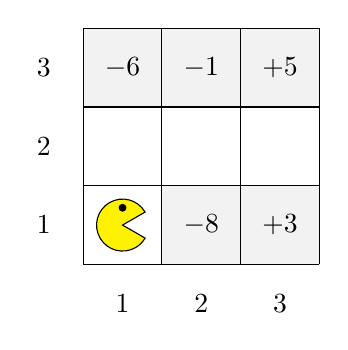
\begin{tikzpicture}
        \draw[step=1cm, black, thin] (0,0) grid (3,3);
        \fill[black, fill opacity=0.05] (1,0) rectangle (3,1);
        \fill[black, fill opacity=0.05] (0,2) rectangle (3,3);

        \draw[black, thin, fill=yellow] (0.5, 0.5) -- ++(30:0.33) arc (30:330:0.33) -- cycle;
        \fill[black] (0.5, 0.72) circle (0.05);

        \draw (0.5, -0.5) node {1};
        \draw (1.5, -0.5) node {2};
        \draw (2.5, -0.5) node {3};
        \draw (-0.5, 0.5) node {1};
        \draw (-0.5, 1.5) node {2};
        \draw (-0.5, 2.5) node {3};

        \draw (1.5, 0.5) node {$-8$};
        \draw (2.5, 0.5) node {$+3$};
        \draw (0.5, 2.5) node {$-6$};
        \draw (1.5, 2.5) node {$-1$};
        \draw (2.5, 2.5) node {$+5$};
    \end{tikzpicture}
    \vspace{-1ex}
\end{figure}

Consider the grid-world given above and an agent who is trying to learn the optimal policy. The agent starts from the bottom-left corner and can take the actions \texttt{north} ($N$), \texttt{south} ($S$), \texttt{west} ($W$) and \texttt{east} ($E$). Rewards are only awarded for reaching the terminal (shaded) states. You observe the following trials, whose trajectories are sequences of tuples $(s^i_t, r^i_t, a^i_t, s^i_{t+1})$.

\begin{table}[h]
    \centering
    \resizebox{0.95\textwidth}{!}{%
    \begin{tabular}{c|ccccc}
        \toprule
         $t$ & Trial 1 & Trial 2 & Trial 3 & Trial 4 & Trial 5 \\
         \midrule
         0 & $(1, 1), 0, N, (1, 2)$ & $(1, 1), 0, N, (1, 2)$ & $(1, 1), 0, N, (1, 2)$ & $(1, 1), 0, N, (1, 2)$ & $(1, 1), 0, N, (1, 2)$ \\
         1 & $(1, 2), 0, E, (2, 2)$ & $(1, 2), 0, E, (2, 2)$ & $(1, 2), 0, E, (2, 2)$ & $(1, 2), 0, E, (2, 2)$ & $(1, 2), 0, E, (2, 2)$ \\
         2 & $(2, 2), 0, N, (2, 3)$ & $(2, 2), 0, E, (3, 2)$ & $(2, 2), 0, S, (2, 1)$ & $(2, 2), 0, E, (3, 2)$ & $(2, 2), 0, E, (3, 2)$ \\
         3 & $(2, 3), -1, \varnothing, \varnothing$ & $(3, 2), 0, N, (3, 3)$ & $(2, 1), -8, \varnothing, \varnothing$ & $(3, 2), 0, W, (2, 2)$ & $(3, 2), 0, S, (3, 1)$ \\
         4 & & $(3, 3), +5, \varnothing, \varnothing$ & & $(2, 2), 0, N, (2, 3)$ & $(3, 1), +3, \varnothing, \varnothing$ \\
         5 & & & & $(2, 3), -1, \varnothing, \varnothing$ & \\
         \bottomrule
    \end{tabular}}
\end{table}

Assuming a discount factor $\gamma = 1$,

\begin{enumerate}
    \item Perform direct utility estimation of the expected utilities $V^\pi(s)$, given the four first trials.

    \begin{solution}
        In this setting, the transition model $P(s' | s, a)$ and the reward function $R(s)$ are unknown. We wish to learn the expected utility $V^\pi$ of the policy $\pi$ without modeling the environment, \ie{} without building approximates $\hat{P}(s' | s, a)$ and $\hat{R}(s)$. The principle of direct utility estimation is to approximate $V^\pi(s)$ by the average utility $\hat{V}(s)$ of the state $s$ within all trial trajectories, \ie{}
        \begin{equation*}
            \hat{V}(s) = \frac{1}{N(s)} \sum_{(i, j) \in I(s)} \sum_{t = 0}^{\infty} \gamma^t r^i_{j + t} \approx V^\pi(s) = \left. \E \sbk*{\sum_{t = 0}^{\infty} \gamma^t R(s_t)} \right|_{s_0 = s}
        \end{equation*}
        where $I(s) = \cbk{(i, j): s^i_j = s}$ indexes the occurrences of $s$ and $N(s) = \abs{I(s)}$ is the number of occurrences of $s$. For examples, in our case and excluding the fifth trial,
        \begin{align*}
            I((1, 1)) & = \cbk{(1, 0), (2, 0), (3, 0), (4, 0)} \\
            \hat{V}((1, 1)) & \approx \frac{1}{4} \rbk*{- 1 \, \gamma^3 + 5 \, \gamma^4 - 8 \, \gamma^3 - 1 \, \gamma^5} = \frac{-5}{4} \\
            I((2, 2)) & = \cbk{(1, 2), (2, 2), (3, 2), (4, 2), (4, 4)} \\
            \hat{V}((2, 2)) & \approx \frac{1}{5} \rbk*{- 1 \, \gamma^1 + 5 \, \gamma^2 - 8 \, \gamma^1 - 1 \, \gamma^3 - 1 \, \gamma^1} = \frac{-6}{5} \\
            I((2, 3)) & = \cbk{(1, 3), (4, 5)} \\
            \hat{V}((2, 3)) & \approx \frac{1}{2} \rbk*{- 1 \, \gamma^0 - 1 \, \gamma^0} = -1 .
        \end{align*}
        Importantly, since the agent hasn't reached the states $(1, 3)$ and $(3, 3)$ yet, it is not possible to estimate their expected utility. Instead, we assume a default value of $0$.

        \begin{figure}[h]
            \centering
            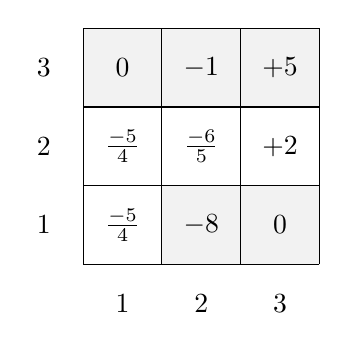
\begin{tikzpicture}
                \draw[step=1cm, black, thin] (0,0) grid (3,3);
                \fill[black, fill opacity=0.05] (1,0) rectangle (3,1);
                \fill[black, fill opacity=0.05] (0,2) rectangle (3,3);

                \draw (0.5, -0.5) node {1};
                \draw (1.5, -0.5) node {2};
                \draw (2.5, -0.5) node {3};
                \draw (-0.5, 0.5) node {1};
                \draw (-0.5, 1.5) node {2};
                \draw (-0.5, 2.5) node {3};

                \draw (0.5, 0.5) node {$\frac{-5}{4}$};
                \draw (1.5, 0.5) node {$-8$};
                \draw (2.5, 0.5) node {0};
                \draw (0.5, 1.5) node {$\frac{-5}{4}$};
                \draw (1.5, 1.5) node {$\frac{-6}{5}$};
                \draw (2.5, 1.5) node {$+2$};
                \draw (0.5, 2.5) node {0};
                \draw (1.5, 2.5) node {$-1$};
                \draw (2.5, 2.5) node {$+5$};
            \end{tikzpicture}
        \end{figure}
    \end{solution}

    \item Update the estimated expected utilities with respect to the fifth trial using temporal-difference learning. Assume a learning rate $\alpha = 0.5$.

    \begin{solution}
        Direct utility estimation misses the fact that the expected utilities for different states are not independent, since they obey the Bellman equation for a fixed policy
        \begin{equation*}
            V^\pi(s) = R(s) + \gamma \sum_{s'} P(s' | s, \pi(s)) V^\pi(s').
        \end{equation*}
        Then, we would like our estimates $\hat{V}(s)$ to verify the Bellman equation, \ie{} to minimize
        \begin{equation*}
            L = \underset{s' | s}{\E} \sbk*{\rbk*{R(s) + \gamma \hat{V}(s') - \hat{V}(s)}^2} .
        \end{equation*}
        One way to reach this objective is to follow the opposite of its gradient
        \begin{equation*}
            \nabla L = 2 \underset{s' | s}{\E} \sbk*{\hat{V}(s) - R(s) - \gamma \hat{V}(s')}
        \end{equation*}
        with respect to $\hat{V}(s)$, \ie{} to perform \emph{gradient descent}. Unfortunately, due to the expectation, we don't have access to the true gradient. Instead, we use a \emph{stochastic} approximation of the gradient from observed\footnotemark{} tuples $(s, r, a, s')$ and update $\hat{V}(s)$ as
        \begin{align*}
            \hat{V}(s) & \gets \hat{V}(s) - \alpha \rbk*{\hat{V}(s) - r - \gamma \hat{V}(s')} \\
            & \gets (1 - \alpha) \hat{V}(s) + \alpha \rbk*{r + \gamma \hat{V}(s')}
        \end{align*}
        where $\alpha$ is the learning rate. For a fixed learning rate, the average of $\hat{V}(s)$ converge towards (oscillates around) the true expected utility $V^\pi(s)$. For a (slowly) decreasing learning rate, $\hat{V}(s)$ itself converges to $V^\pi(s)$. For historical reasons, this algorithm is called temporal-difference (TD) learning.

        \footnotetext{We are not limited to perform only one update for each tuple $(s, r, a, s')$. Indeed, as we assume the policy to be stationary, past trials are as likely to happen again as more recent ones. Therefore, reusing tuples several times (in other orders) is a good way to improve estimates while generating less trials.}

        Following the trajectory of the fifth trial, we perform the updates
        \begin{align*}
            V^\pi((1, 1)) & \gets (1 - \alpha) V^\pi((1, 1)) + \alpha \rbk*{0 + \gamma V^\pi((1, 2))} = \frac{1}{2} \frac{-5}{4} + \frac{1}{2} \frac{-5}{4} = \frac{-5}{4} \\
            V^\pi((1, 2)) & \gets (1 - \alpha) V^\pi((1, 2)) + \alpha \rbk*{0 + \gamma V^\pi((2, 2))} = \frac{1}{2} \frac{-5}{4} + \frac{1}{2} \frac{-6}{5} = \frac{-49}{40} \\
            V^\pi((2, 2)) & \gets (1 - \alpha) V^\pi((2, 2)) + \alpha \rbk*{0 + \gamma V^\pi((3, 2))} = \frac{1}{2} \frac{-6}{5} + \frac{1}{2} 2 = \frac{+4}{10} \\
            V^\pi((3, 2)) & \gets (1 - \alpha) V^\pi((3, 2)) + \alpha \rbk*{0 + \gamma V^\pi((3, 1))} = \frac{1}{2} 2 + \frac{1}{2} 0 = +1 \\
            V^\pi((3, 1)) & \gets (1 - \alpha) V^\pi((3, 1)) + \alpha \rbk*{3 + 0} = \frac{1}{2} 0 + \frac{1}{2} 3 = \frac{+3}{2} .
        \end{align*}

        \begin{figure}[h]
            \centering
            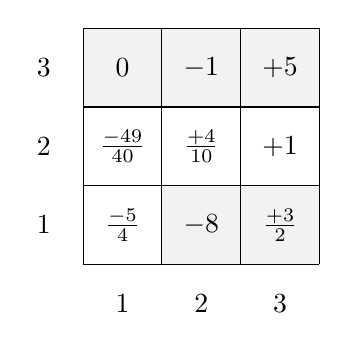
\begin{tikzpicture}
                \draw[step=1cm, black, thin] (0,0) grid (3,3);
                \fill[black, fill opacity=0.05] (1,0) rectangle (3,1);
                \fill[black, fill opacity=0.05] (0,2) rectangle (3,3);

                \draw (0.5, -0.5) node {1};
                \draw (1.5, -0.5) node {2};
                \draw (2.5, -0.5) node {3};
                \draw (-0.5, 0.5) node {1};
                \draw (-0.5, 1.5) node {2};
                \draw (-0.5, 2.5) node {3};

                \draw (0.5, 0.5) node {$\frac{-5}{4}$};
                \draw (1.5, 0.5) node {$-8$};
                \draw (2.5, 0.5) node {$\frac{+3}{2}$};
                \draw (0.5, 1.5) node {$\frac{-49}{40}$};
                \draw (1.5, 1.5) node {$\frac{+4}{10}$};
                \draw (2.5, 1.5) node {$+1$};
                \draw (0.5, 2.5) node {0};
                \draw (1.5, 2.5) node {$-1$};
                \draw (2.5, 2.5) node {$+5$};
            \end{tikzpicture}
        \end{figure}
    \end{solution}
\end{enumerate}

\newpage

\section{Football}

\def\C{\texttt{C}}
\def\A{\texttt{A}}
\def\F{\texttt{F}}
\def\G{\texttt{G}}
\def\P{\texttt{P}}
\def\S{\texttt{S}}

ULiège's football team is playing against UCL's team next week. With a lot of losses this season, Liège needs to improve their attack strategy to win the game and increase their popularity. Luckily, the team captain follows INFO8006 and knows how to model the attack as a Markov Decision Process. The captain considers four states \texttt{close} (\C), \texttt{away} (\A), \texttt{fail} (\F), and \texttt{goal} (\G), and two actions \texttt{pass} (\P) and \texttt{shoot} (\S). Although the transition probabilities are unsure, the possible transitions $(s, a, s')$ are known. To each transition is associated an increase/decrease of the team's popularity.

\begin{table}[h]
    \centering
    \begin{tabular}{ccc|c}
        \toprule
         $s$ & $a$ & $s'$ & $R(s, a, s')$ \\
         \midrule
         \C & \P & \C & $+1$ \\
         \C & \P & \A & $-1$ \\
         \C & \P & \F & $-2$ \\
         \C & \S & \C & $+3$ \\
         \C & \S & \F & $-5$ \\
         \C & \S & \G & $+10$ \\
         \midrule
         \A & \P & \C & $+2$ \\
         \A & \P & \A & $0$ \\
         \A & \P & \F & $-3$ \\
         \A & \S & \C & $+3$ \\
         \A & \S & \F & $-10$ \\
         \A & \S & \G & $+20$ \\
         \bottomrule
    \end{tabular}
\end{table}

The current strategy of the team is to always shoot. Last match, they had several attack opportunities, resulting in the following actions.

\begin{table}[h]
    \centering
    \begin{tabular}{c|cccccccc}
        \toprule
         $s$ & \C & \C & \C & \C & \A & \A & \A & \A \\
         $a$ & \S & \S & \S & \S & \S & \S & \S & \S \\
         $s'$ & \G & \C & \G & \F & \F & \C & \F & \F \\
         \bottomrule
    \end{tabular}
\end{table}

Assuming a discount factor $\gamma = 0.75$ and a learning rate $\alpha = 0.25$,

\begin{enumerate}
    \item Build an estimator of the transition model $P(s' | s, a)$ and, from it, determine the expected utility $V^\pi$ of the team's current policy $\pi$.
    \begin{solution}
        Given the previous table, we can estimate the transition probabilities for $s \in \cbk{\C, \A}$ and $a = \S$.

        \begin{table}[h]
            \centering
            \begin{tabular}{cc|cccc}
                \toprule
                 $s$ & $a$ & \multicolumn{4}{c}{$P(s' | s, a)$} \\
                     &     & \C & \A & \F & \G \\
                 \midrule
                 \C & \S & $0.25$ & $0$ & $0.25$ & $0.5$ \\
                 \A & \S & $0.25$ & $0$ & $0.75$ & $0$ \\
                 \bottomrule
            \end{tabular}
        \end{table}

        We can now determine the expected utility $V^\pi$ of the team's current policy $\pi(s) = \S$ using the following Bellman operator
        \begin{equation*}
            V_{i + 1}^\pi(s) = \sum_{s'} P(s' | s, \pi(s)) \sbk*{R(s, \pi(s), s') + \gamma V_i^\pi(s')} ,
        \end{equation*}
        with $V_0^\pi(s) = 0$ for all state $s$. Because the states \F and \G are terminal, their expected utility remains constant and we only have to update \C and \A. For the first iteration,
        \begin{align*}
            V_1^\pi(\C) & = \sum_{s'} P(s' | \C, \S) \sbk*{R(\C, \S, s') + \gamma V_0^\pi(s')} \\
            & = 0.25 (3 + \gamma \, 0) + 0.25 (-5 + \gamma \, 0) + 0.5 (10 + \gamma \, 0) = 4.5
        \end{align*}
        and
        \begin{align*}
            V_1^\pi(\A) & = \sum_{s'} P(s' | \A, \S) \sbk*{R(\A, \S, s') + \gamma V_0^\pi(s')} \\
            & = 0.25 (3 + \gamma \, 0) + 0.75 (-10 + \gamma \, 0) = -6.75 .
        \end{align*}
        We repeat the same procedure until $V_{i + 1}^\pi(s) \approx V_i^\pi(s)$ for all state $s$.

        \begin{table}[h]
            \centering
            \begin{tabular}{c|cccc}
                \toprule
                $s$ & \C & \A & \F & \G \\
                \midrule
                $V_0^\pi(s)$ & 0 & 0 & 0 & 0 \\
                $V_1^\pi(s)$ & 4.5 & -6.75 & 0 & 0 \\
                $V_2^\pi(s)$ & \num{5.3437} & \num{-5.9063} & 0 & 0 \\
                $V_3^\pi(s)$ & \num{5.5019} & \num{-5.7480} & 0 & 0 \\
                $V_4^\pi(s)$ & \num{5.5316} & \num{-5.7183} & 0 & 0 \\
                \vdots       & \vdots & \vdots & \vdots & \vdots \\
                $V_8^\pi(s)$ & \num{5.5385} & \num{-5.7115} & 0 & 0 \\
                \bottomrule
            \end{tabular}
        \end{table}
    \end{solution}

\end{enumerate}

The captain found the tapes of the previous season where they had much more success. Together with the team, the captain selects the following instructive actions.

\begin{table}[h]
    \centering
    \begin{tabular}{c|cccccccc}
        \toprule
         $s$ & \C & \C & \A & \A & \C & \A & \A & \C \\
         $a$ & \S & \S & \S & \P & \P & \P & \S & \P \\
         $s'$ & \G & \C & \F & \C & \C & \C & \F & \F \\
         \bottomrule
    \end{tabular}
\end{table}

\begin{enumerate}
    \setcounter{enumi}{1}
    \item Given the selected tuples, apply the $Q$-learning algorithm to obtain state-action-value $Q(s, a)$ estimates. Estimates are initialized to 0.

    \begin{solution}
        In $Q$-learning, the state-action-value $Q(s, a)$ estimates are updated following
        \begin{align*}
            Q(s, a) & \gets Q(s, a) - \alpha \rbk*{Q(s, a) - r - \gamma \max_{a'} Q(s', a')} \\
            & \gets (1 - \alpha) Q(s, a) + \alpha \rbk*{r + \gamma \max_{a'} Q(s', a')}
        \end{align*}
        for observed tuples $(s, r, a, s')$. In our case, we have a list a 16 (8 + 8) tuples $(s, a, s')$ and we have access to the reward function $R(s, a, s')$. Using the tuples in arbitrary order, we have
        \begin{align*}
            Q(\C, \S) & \gets (1 - \alpha) Q(\C, \S) + \alpha \rbk*{R(\C, \S, \G) + \gamma \max_{a'} Q(\G, a')} \\
            & \gets 0.75 \times 0 + 0.25 \rbk{10 + 0} = 2.5 \\
            Q(\C, \S) & \gets (1 - \alpha) Q(\C, \S) + \alpha \rbk*{R(\C, \S, \C) + \gamma \max_{a'} Q(\C, a')} \\
            & \gets 0.75 \times 2.5 + 0.25 \rbk{3 + 0.75 \max \cbk{2.5, 0}} = 3.094 \\
            Q(\A, \S) & \gets (1 - \alpha) Q(\A, \S) + \alpha \rbk*{R(\A, \S, \F) + \gamma \max_{a'} Q(\F, a')} \\
            & \gets 0.75 \times 0 + 0.25 \rbk{-10 + 0} = -2.5 \\
            Q(\A, \P) & \gets (1 - \alpha) Q(\A, \P) + \alpha \rbk*{R(\A, \P, \C) + \gamma \max_{a'} Q(\C, a')} \\
            & \gets 0.75 \times 0 + 0.25 \rbk{2 + 0.75 \max \cbk{3.094, 0}} = 4.320 \\
            Q(\C, \P) & \gets \dots
        \end{align*}
    \end{solution}

    \item Determine the optimal policy according to the state-action-value estimates.

    \begin{solution}
        \begin{equation*}
            \pi(s) = \begin{cases}
                \S & \text{if } s = \C \\
                \P & \text{if } s = \A
            \end{cases}
        \end{equation*}
    \end{solution}
\end{enumerate}

\newpage

\part*{Supplementary exercises}

\section{(AIMA, Ex 16.15)}

Consider a student, Sam, who has the choice to buy or not buy a textbook for a course. We'll model this as a decision problem with one Boolean decision node, $B$, indicating whether the agent chooses to buy the book, and two Boolean chance nodes,
$M$, indicating whether the student has mastered the material of the course, and $F$, indicating whether the student fails the course. There is also a utility node, $U$. Sam has an additive utility function: 0 for not buying the book and \qty{-100}{\$} for buying it; and 0 for failing the course and \qty{2000}{\$} for passing it. Sam's conditional probability estimates are as follows:

\begin{table}[h]
    \centering
    \begin{tabular}{cc|cc}
        \toprule
        $B$ & $M$ & $P(M | B)$ & $P(F = 1 | B, M)$ \\
        \midrule
        0 & 0 & 0.3 & 0.7 \\
        1 & 0 & 0.1 & 0.5 \\
        0 & 1 & 0.7 & 0.2 \\
        1 & 1 & 0.9 & 0.1 \\
        \bottomrule
    \end{tabular}
\end{table}

\begin{enumerate}
    \item Draw the decision network for this problem.

    \item Compute the expected utility of buying the book and of not buying it.

    \item What should Sam do?
\end{enumerate}

\newpage

\section{(AIMA, Ex 17.6)}

The slides of the course states that the Bellman operator
\begin{equation*}
    (B V)(s) = R(s) + \gamma \max_{a \in A(s)} \sum_{s'} P(s' | s, a) V(s')
\end{equation*}
is a contraction.

\begin{enumerate}
    \item Show that, for any two functions $f: \R \mapsto \R$ and $g: \R \mapsto \R$,
    \begin{equation*}
        \abs{\max_x f(x) - \max_x g(x)} \leq \max_x \, \abs{f(x) - g(x)} .
    \end{equation*}

    \item Apply the previous result to prove that the Bellman operator is a contraction of factor $\gamma$, that is
    \begin{equation*}
        \norm{(BV) - (BV')}_\infty \leq \gamma \norm{V - V'}_\infty .
    \end{equation*}
    \blindfootnote{The infinity norm of a function $f: \R \mapsto \R$ is defined as
    \begin{equation*}
        \norm{f}_\infty = \sup_x \abs{f(x)} .
    \end{equation*}}
\end{enumerate}

\newpage

\section{(AIMA, Ex 17.8)} \label{sec:17.8}

Consider the $3 \times 3$ world shown in Figure \ref{fig:grid-mdp}. The transition model is the same as in the $4 \times 3$ \ref{fig:sequential}: \qty{80}{\percent} of the time the agent goes in the direction it selects; the rest of the time it moves at right angles to the intended direction.

\begin{figure}[h]
    \centering
    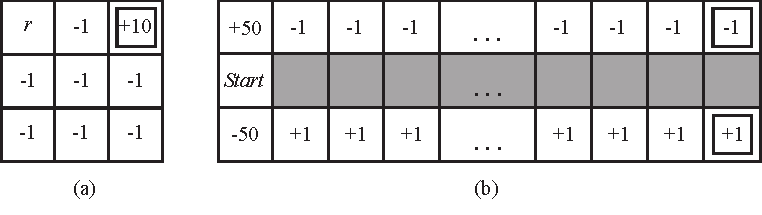
\includegraphics{figures/e6_grid_mdp.pdf}
    \caption{(a) $3\times3$ world for \ref{sec:17.8}. The reward for each state is indicated. The upper right square is a terminal state. (b) $101 \times 3$ world for \ref{sec:17.9}. The start state has reward $0$.}
    \label{fig:grid-mdp}
\end{figure}

\begin{figure}[h]
    \centering
    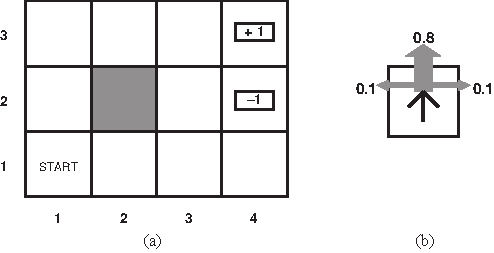
\includegraphics{figures/e6_sequential.pdf}
    \caption{(a) A simple $4\times 3$ environment that presents the agent with a sequential decision problem. The two terminal states have reward $+1$ and $-1$, respectively, and all other states have a reward of $-0.04$. (b) Illustration of the transition model of the environment: the \enquote{intended} outcome occurs with probability $0.8$, but with probability $0.2$ the agent moves at right angles to the intended direction. A collision with a wall results in no movement.}
    \label{fig:sequential}
\end{figure}

Implement value iteration for this world for each value of $r$ below. Use discounted rewards with a discount factor $\gamma = \num{0.99}$. Show
the policy obtained in each case. Explain intuitively why the value of $r$ leads to each policy.

\begin{enumerate}
    \item $r = -100$
    \item $r = -3$
    \item $r = 0$
    \item $r = +3$
\end{enumerate}

\newpage

\section{(AIMA, Ex 17.9)} \label{sec:17.9}

Consider the $101 \times 3$ world shown in Figure \ref{fig:grid-mdp}. In the start state the agent has a choice of two deterministic actions, \texttt{up} or \texttt{down}, but in the other states the agent has one deterministic action, \texttt{right}. Assuming a discounted reward function, compute the utility of each action as a function of $\gamma$. For what values of the discount factor $\gamma$ should the agent choose \texttt{up} and for which \texttt{down}?

\blindfootnote{This simple example actually reflects many real-world situations in which one must weigh the value of an immediate action versus the potential long-term consequences, such as choosing to dump pollutants into a lake.}

\newpage

\section{(AIMA, Ex 17.10)}

Consider an undiscounted MDP having three states, $(1, 2, 3)$, with rewards $-1$, $-2$, $0$, respectively. State 3 is a terminal state. In states 1 and 2 there are two possible actions: $a$ and $b$. The transition model is as follows:

\begin{itemize}
    \item In state 1, action $a$ moves the agent to state 2 with probability $0.8$ and makes the agent stay put with probability $0.2$.
    \item In state 2, action $a$ moves the agent to state 1 with probability $0.8$ and makes the agent stay put with probability 0.2.
    \item In either state 1 or state 2, action $b$ moves the agent to state 3 with probability $0.1$ and makes the agent stay put with probability $0.9$.
\end{itemize}

Answer the following questions:

\begin{enumerate}
    \item What can be determined \emph{qualitatively} about the optimal policy in states 1 and 2?

\begin{comment}
    \begin{solution}
         Intuitively, the agent wants to get to state 3 as soon as possible, because it will pay a cost for each time step it spends in states 1 and 2. However, the only action that reaches state 3 (action b) succeeds with low probability, so the agent should minimize the cost it incurs while trying to reach the terminal state. This suggests that the agent should definitely try action $b$ in state 1, but, in state 2, it might be better to try action $a$ to get to state 1, rather than aiming directly for state 3. The decision in state 2 involves a numerical trade-off.
    \end{solution}
\end{comment}

    \item Apply policy iteration, showing each step in full, to determine the optimal policy and the values of states 1 and 2. Assume that the initial policy has action $b$ in both states.

\begin{comment}
    \begin{solution}
        \begin{itemize}
            \item Initialization: $R \leftarrow\langle- 1,-2,0\rangle, \pi^0 \leftarrow\langle b, b\rangle$.
            \item Value determination:
            $$
            \begin{array}{l}{V(s_{1})=-1+0.1 V(s_{3})+0.9 V(s_{1})} \\ {V(s_{2})=-2+0.1 V(s_{3})+0.9 V(s_{2})} \\ {V(s_{3})=0}\end{array}
            $$
            That is, $V(s_1) =-10$ and $V(s_2) =-20$.
            Policy update:
            \begin{itemize}
                \item In state 1,
                $\pi^1(s_1) = a$ leads to $\sum_{i \in \{1, 2, 3\}} P(s_i|s_1, a) V(s_i) = 0.8 \times -20 + 0.2 \times -10 = -18$ and $\pi^1(s_1) = b$ leads $\sum_{i \in \{1, 2, 3\}} P(s_i|s_1, b) V(s_i)  = 0.1 \times 0 + 0.9 \times -10 = -9$, thus $\pi^1(s_1) = b$.

                \item In state 2,
                $\pi^1(s_2) = a$ leads to $\sum_{i \in \{1, 2, 3\}} P(s_i|s_2, a) V(s_i) = 0.2 \times -20 + 0.8 \times -10 = -12$ and $\pi^1(s_2) = b$ leads $\sum_{i \in \{1, 2, 3\}} P(s_i|s_2, b) V(s_i)  = 0.1 \times 0 + 0.9 \times -20 = -18$, thus $\pi^1(s_2) = a$.
            \end{itemize}
            \item Value determination:
            $$
            \begin{array}{l}{V(s_{1})=-1+0.1 V(s_{3})+0.9 V(s_{1})} \\ {V(s_{2})=-2+0.8 V(s_{1})+0.2 V(s_{2})} \\ {V(s_{3})=0}\end{array}
            $$
            That is, $V(s_1) =-10$ and $V(s_2) = -12.5$.
            Policy update:
            \begin{itemize}
                \item In state 1,
                $\pi^1(s_1) = a$ leads to $\sum_{i \in \{1, 2, 3\}} P(s_i|s_1, a) V(s_i) = 0.8 \times -12.5 + 0.2 \times -10 = -12$ and $\pi^1(s_1) = b$ leads $\sum_{i \in \{1, 2, 3\}} P(s_i|s_1, b) V(s_i)  = 0.1 \times 0 + 0.9 \times -10 = -9$, thus $\pi^1(s_1) = b$.

                \item In state 2,
                $\pi^1(s_2) = a$ leads to $\sum_{i \in \{1, 2, 3\}} P(s_i|s_2, a) V(s_i) = 0.2 \times -12.5 + 0.8 \times -10 = -10.5$ and $\pi^1(s_2) = b$ leads $\sum_{i \in \{1, 2, 3\}} P(s_i|s_2, b) V(s_i)  = 0.1 \times 0 + 0.9 \times -12.5 = -11.25$, thus $\pi^1(s_2) = a$.
            \end{itemize}
            \item Unchanged, which implies convergence.
        \end{itemize}
    \end{solution}
\end{comment}

    \item What happens to policy iteration if the initial policy has action $a$ in both states? Does discounting help? Does the optimal policy depend on the discount factor?

\begin{comment}
    \begin{solution}
        An initial policy with action $a$ in both states leads to an unsolvable problem. The initial value determination problem has the form $$\begin{array}{l}{u_{1}=-1+0.2 u_{1}+0.8 u_{2}} \\ {u_{2}=-2+0.8 u_{1}+0.2 u_{2}} \\ {u_{3}=0}\end{array}$$ and the first two equations are inconsistent. If we were to try to solve them iteratively, we would find the values tending to $-\infty$. Discounting leads to well-defined solutions by bounding the penalty (expected dis- counted cost) an agent can incur at either state. However, the choice of discount factor will affect the policy that results. For $\gamma$ small, the cost incurred in the distant future plays a negligible role in the value computation, because $\gamma^n$ is near $0$. As a result, an agent could choose action $b$ in state 2 because the discounted short-term cost of remaining in the non-terminal states (states 1 and 2) outweighs the discounted long-term cost of action $b$ failing repeatedly and leaving the agent in state 2.
    \end{solution}
\end{comment}
\end{enumerate}

\newpage

\section{(AIMA, Ex 17.19)}

A Dutch auction is similar to an English auction, but rather than starting the bidding at a low price and increasing, the seller starts at a high price and gradually lowers the price until some buyer is willing to accept that price. If multiple bidders accept the price, one is arbitrarily chosen as the winner. More formally, the seller begins with a price $p$ and gradually lowers $p$ by increments of $d$ until at least one buyer accepts the price.

Assuming all bidders act rationally, is it true that for arbitrarily small $d$, a Dutch auction will always result in the bidder with the highest value for the item obtaining the item? If so, show mathematically why. If not, explain how it may be possible for the bidder with highest value for the item not to obtain it.

\newpage

\section{(AIMA, Ex 17.21)}

Teams in the National Hockey League historically received 2 points for winning a game and 0 for losing. If the game is tied, an overtime period is played; if nobody wins in overtime, the game is a tie and each team gets 1 point. But league officials felt that teams were playing too conservatively in overtime (to avoid a loss), and it would be more exciting if overtime produced a winner. So in 1999 the officials experimented in mechanism design: the rules were changed, giving a team that loses in overtime 1 point, not 0. It is still 2 points for a win and 1 for a tie.

\begin{enumerate}
    \item Was hockey a zero-sum game before the rule change? After?

    \item Suppose that at a certain time $t$ in a game, the home team has probability $p$ of winning in regulation time, probability $0.78 - p$ of losing, and probability $0.22$ of going into overtime, where they have probability $q$ of winning, $0.9 - q$ of losing, and $0.1$ of tying. Give equations for the expected value for the home and visiting teams.

    \item Imagine that it were legal and ethical for the two teams to enter into a pact where they agree that they will skate to a tie in regulation time, and then both try in earnest to win in overtime. Under what conditions, in terms of $p$ and $q$, would it be rational for both teams to agree to this pact?

    \item Some experts report that since the rule change, the percentage of games with a winner in overtime went up \qty{18.2}{\percent}, as desired, but the percentage of overtime games also went up \qty{3.6}{\percent}. What does that suggest about possible collusion or conservative play after the rule change?
\end{enumerate}

\newpage

\startquiz
Which of the following is true? In Markov Decision Processes, ...
\begin{itemize}
    \item the closer the discount factor $\gamma$ to $0$, the higher the utility of future rewards.
    \item the closer the discount factor $\gamma$ to $0$, the longer Value Iteration may take to converge. 
    \item the closer the discount factor $\gamma$ to $1$, the greedier the optimal agent. 
    \solitem the closer the discount factor $\gamma$ to $1$, the longer Value Iteration may take to converge.  %%%
\end{itemize}
Q-Learning ...
\begin{itemize}
    \item is a model-based reinforcement learning algorithm.
    \item is an on-policy reinforcement learning algorithm.
    \item converges to an optimal policy, but only when acting optimally.
    \solitem requires a random exploration strategy to converge to an optimal policy. %%%
\end{itemize}
Assume that we run $\epsilon$-greedy Q-learning until convergence. What is the optimal policy $\pi^*$ we obtain for an arbitrary state $s$?
\begin{itemize}
    \item $\pi^*(s) = \arg\max_s V(s)$
    \item $\pi^*(s) = \begin{cases}
        \arg\max_a Q(s,a) & \text{with probability $1-\epsilon$}\\
        \text{random action} & \text{with probability $\epsilon$}
    \end{cases}$
    \solitem $\pi^*(s) = \arg\max_a Q(s,a)$ %%%
    \item $\pi^*(s) = \arg\max_s Q(s,a)$
\end{itemize}
Let us consider a robot wandering around at the Montefiore Institute. Which of the following is true?
\begin{itemize}
    \solitem The robot and its environment can be modeled as a partially observable MDP. %%%%
    \item The Kalman filter can be used for determining accurately its past trajectory in the building. 
    \item A convolutional neural network would be too large to fit in the robot's memory.
    \item Value iteration (with an admissible heuristic) can be used for decoding the speech of its visitors.
\end{itemize}
The Bellman equations $Q(s,a) = R(s) + \gamma \sum_{s'} P(s'|s,a) \max_{a'} Q(s',a')$ form a system of $n$ non-linear equations with as many unknowns. Which of the following is true?
\begin{itemize}
    \item $n$ is the size of the action space $\mathcal{A}$.
    \item $n$ is the size of the state space $\mathcal{S}$.
    \solitem $n$ is the size of the state-action space $\mathcal{S} \times \mathcal{A}$. %%%
    \item $n$ is the sum of the sizes of the action and state spaces.
\end{itemize}
In DQN (Mnih et al, 2015), a reinforcement learning agent is trained to ...
\begin{itemize}
    \item to classify images. 
    \item to control a robot in a simulated environment.
    \solitem to play Atari video games.  %%%
    \item to play the game of Go.
\end{itemize}
In DQN (Mnih et al, 2015), the Q-table is approximated with ...
\begin{itemize}
    \item a hash table.
    \item a transposition table.
    \item a linear regression model.
    \solitem a convolutional neural network. %%%%
\end{itemize}

\end{document}
